\documentclass[APA,Times1COL]{WileyNJDv5} %STIX1COL,STIX2COL,STIXSMALL

\usepackage{threeparttable}
\usepackage{dcolumn}
\usepackage{placeins}
\usepackage{subcaption}
\usepackage{graphicx}%

\graphicspath{{../Figs/}}

\articletype{Original Article}%

\received{Date Month Year}
\revised{Date Month Year}
\accepted{Date Month Year}
\journal{Real Estate Econ.}
\volume{00}
\copyyear{2025}
\startpage{1}

\raggedbottom



\begin{document}

\title{A Novel Proxy of Latent Rental Housing Demand: Evidence from US Markets}

\author[1]{Matt Larriva, CFA}


\authormark{}
\titlemark{Density Shift as a Measure of Demand}

\address[1]{\orgdiv{Department of Real Estate Investments}, \orgname{Brookfield Asset Management}, \orgaddress{\state{New York}, \country{United States}}}



\corres{\email{matt.larriva@brookfield.com}}

\presentaddress{250 Vesey Street, New York NY 10281 }

%\fundingInfo{Text}
%\JELinfo{ejlje}

\abstract[Abstract]{We introduce the Rental Density Index (RDI)---a metric that captures the number of people per rental unit---as a scalable and behaviorally grounded proxy for latent rental housing demand. Traditional demand indicators like occupancy or absorption are bounded by supply and often fail to reflect underlying crowding pressure. In contrast, changes in RDI (\( \Delta \text{RDI} \)) reveal when renters are consolidating space, signaling excess demand, or spreading out, signaling slack.	Using panel data for the 100 largest U.S. metropolitan areas from 2000 to 2024, we show that \( \Delta \text{RDI} \) robustly predicts future rent growth. A two-stage least squares model, instrumenting for RDI growth with plausibly exogenous foreign in-migration shocks, reveals a positive and statistically significant causal effect on next-year relative rent growth. Out-of-sample tests further show that RDI-based forecasts outperform ARIMA and naïve models across one-, five-, and ten-year horizons. Event studies and regime classifications confirm that crowding transitions are consistently followed by directional rent changes.	The Rental Density Index provides a simple yet powerful tool for identifying housing market tightness, classifying supply-demand regimes, and forecasting rent performance. It is especially useful in contexts where traditional demand indicators are constrained or unavailable.}
	


\keywords{density, supply and demand, multifamily rent-growth, apartment markets}

%\jnlcitation{\cname{%	
%\author{Larriva M.}
%\author{}.}
%\ctitle{Density Shift as a Measure of Demand} \cjournal{\it Real Estate Econ.}
%\cvol{2021;00(00):1--18}.}


\maketitle

\renewcommand\thefootnote{}
\footnotetext{\textbf{Abbreviations:} MSA, Metropolitan Statistical Area; RDI, relative density index; }

\renewcommand\thefootnote{\fnsymbol{footnote}}
\setcounter{footnote}{1}
\FloatBarrier
\section{Introduction}\label{sec1}
Housing shortages and affordability concerns have risen to the forefront of policy debates in major urban markets. In the United States, housing production has consistently lagged population growth for decades, contributing to an estimated national shortfall of 4.4 million housing units \cite{betancourt2022us}. Nearly half of U.S. renter households now spend over 30\% of their income on housing \cite{censusNearlyHalf}, and from 2000 to 2024, the consumer price index (CPI) for shelter exceeded the CPI for all other items by 30\% \cite{stlouisfedConsumerPrice}. At the same time, select high-growth regions have recently experienced rent declines due to a glut of new supply \cite{mott2024ThisRegion}. This juxtaposition of chronic national undersupply with localized oversupply underscores a deeper issue: the lack of a reliable metric to measure consumer housing demand.

Traditional indicators of demand in multifamily real estate, such as occupancy rates and net absorption, are informative but fundamentally supply-constrained. Occupancy rates are naturally bounded at 100\%, and absorption cannot exceed the rate of new deliveries \cite{mueller1999real}. These constraints obscure excess demand: when all available and affordable units are occupied, latent demand becomes invisible to market participants and researchers alike \cite{gabriel2001rental, sirmans1991determinants, pyhrr1999real}. This problem inhibits clear attribution of rent increases to supply versus demand dynamics \cite{pennington2021does, molloy2022housing}. Moreover, ongoing academic debate persists around whether rising rents in constrained markets result more from supply-side limitations \cite{saiz2010geographic} or from heightened demand for desirable locations \cite{davidoff2015supply}. Without a transparent, consistent demand-side metric, attempts to assess equilibrium conditions remain incomplete.

In this paper, we introduce a novel empirical measure of rental housing demand: the \textit{rental density index} (RDI), defined as the number of people per existing rental unit in a given metropolitan area. Unlike occupancy or absorption, RDI is not inherently bounded and therefore can reflect intensifying demand even in fully occupied markets. The conceptual foundation is straightforward: as rents rise, renters economize on space---whether by delaying household formation, taking on roommates, or crowding---thus increasing the ratio of people per rental unit. By observing shifts in RDI over time, we capture underlying demand pressures that traditional metrics obscure.

Present trends support this reframing of demand, as density, rental prices, and rental preferences have all shifted meaningfully. For most of its history, the U.S. was less densely populated than its high-income peers, but in 1992 this changed. In that year, the US grew to 28 people per square kilometer, outpacing the High Income countries whose average was 23 people per square kilometer \cite{worldbankPopDensity}. The most recent figures report the US with a density of 36 and the High Income nations with an average density of 27.  Over this same period, rental prices have outpaced both wages and non-shelter inflation \cite{feiveson2024rent, stlouisfedConsumerPrice}, with younger cohorts increasingly preferring rental housing \cite{fanniemaeConsumersFeeling}.

Prior literature in urban economics and real estate has studied density extensively, often linking increased geographic density to higher wages, rents, and productivity due to agglomeration effects \cite{titman2024city, liu2018vertical}. However, these studies generally define density in terms of spatial density: people per square mile or  apartments per square mile. Our focus differs: we define density as the quotient of population over occupied rental units, which provides a clearer window into the number of people actively competing for housing. Unlike geographic density, this measure is directly responsive to shifts in demand, especially during periods of supply constraint or shocks. 

Our framework builds on the standard assumption that, all else equal, households derive higher utility from larger living spaces \cite{muth1969cities,molloy2022housing}. In high-rent markets, however, the extra price per square foot may eventually exceed the marginal benefit of additional space. To economize, renters may respond by sharing units (adding roommates), downsizing to smaller apartments, or relocating to less expensive regions. Conversely, when real rents fall or new supply comes online, the marginal cost of extra space might drop below its marginal utility, enticing households to spread out, move to larger units, or reduce unit‐share.The aggregate effect of these choices combined with the new supply additions or subtractions determines the direction the Rental Density Index change. Because the RDI directly captures these space‐consumption margins, year‐over‐year changes in RDI proxy for shifts in aggregate housing demand at prevailing prices.

\begin{figure}[htb!]
	\centerline{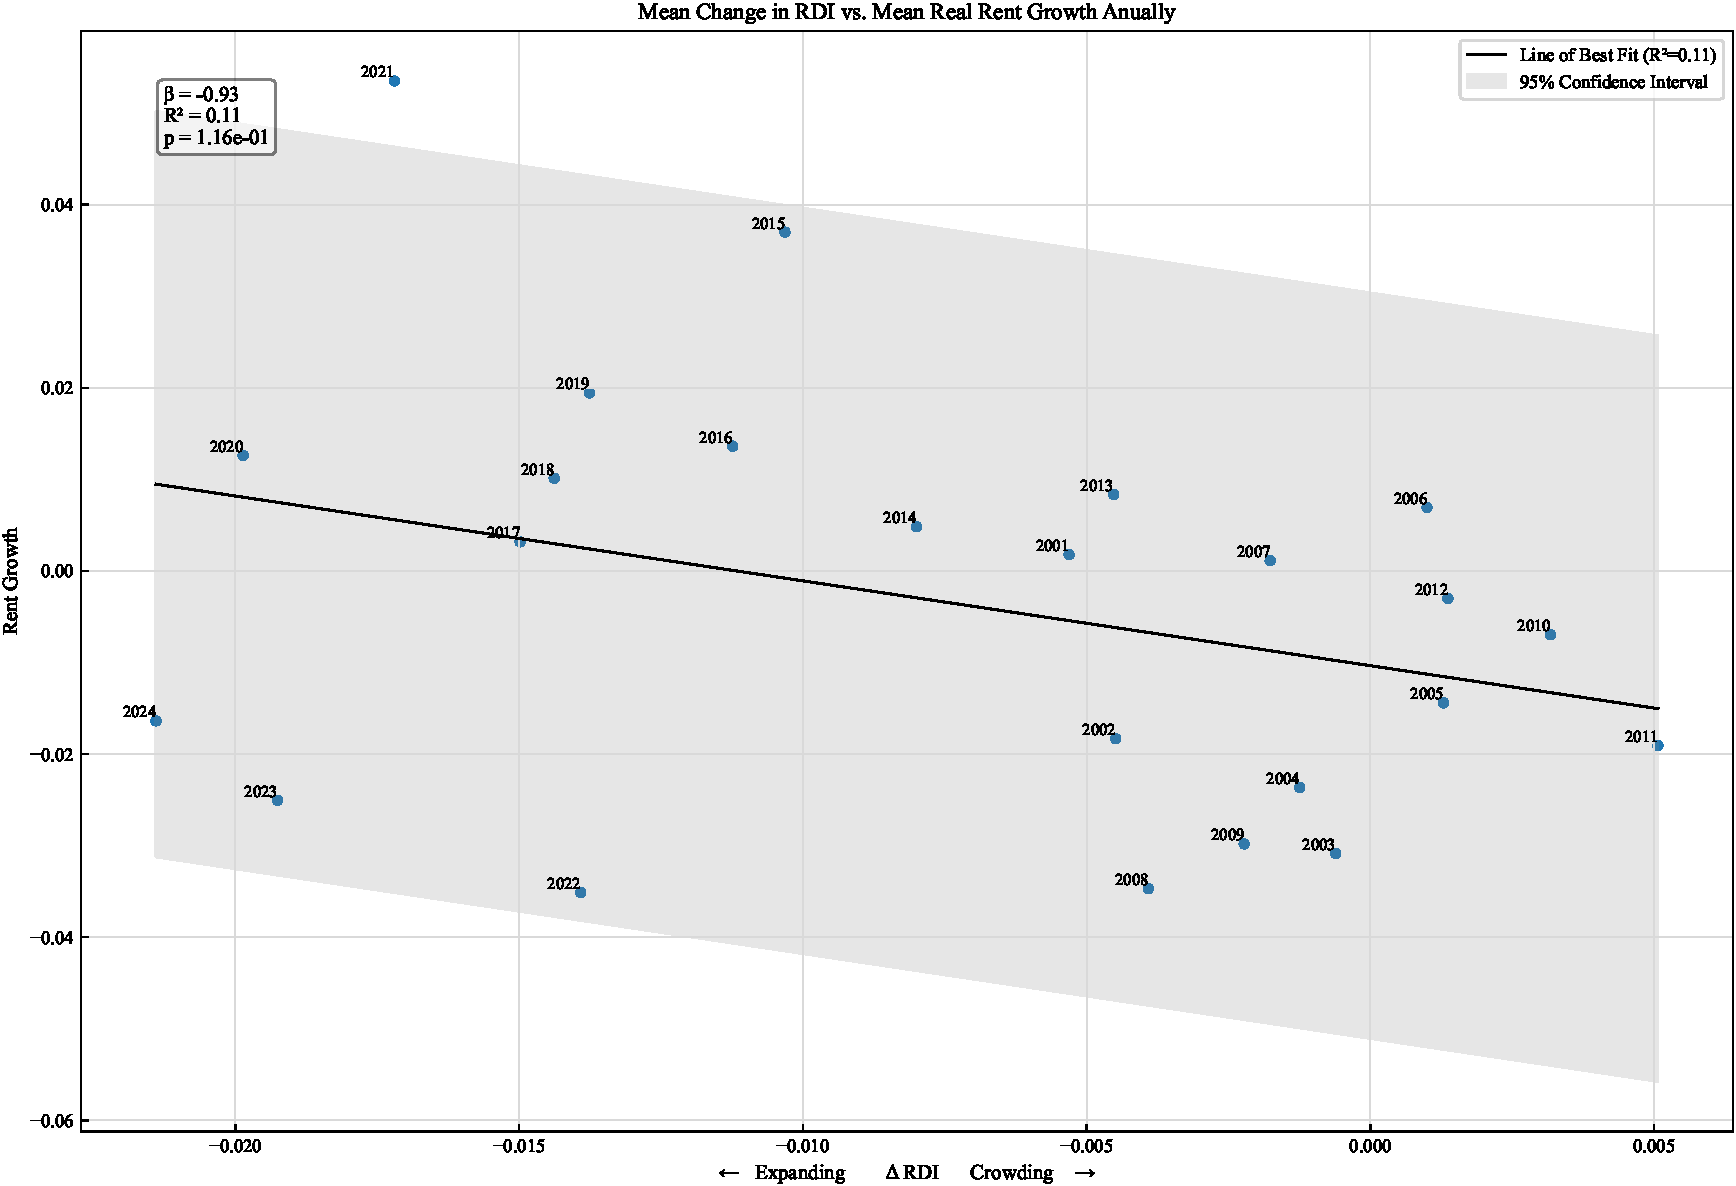
\includegraphics[height=20pc]{rdi_rent_growth_2024.pdf}}
	\caption{Relationship between average annual change in Rental Density Index (horizontal) and average annual relative real rent growth (vertical) in the 100 largest MSAs for each year between 2001 and 2024. \label{fig:rdi_national}}
\end{figure}

Focusing on a panel of the 100 largest metropolitan statistical areas (MSA) between 2000 and 2024, we calculate the RDI. We then examine the year-over-year change in each MSA, in each year. A positive change in RDI (densification) means that population has grown faster than inventory; conversely a negative change in RDI (de-densification) corresponds to inventory growing faster than population. While this ignores the number of households and the percentage of owners versus renters, the signal from the RDI change is robust in spite of this.

This empirical strategy reveals consistent rent growth differences across multiple time horizons. Over the one-year horizon, top RDI growth  markets significantly outperform the bottom RDI growth quintile markets. The densifying markets outperform the de-densifying markets by over 100 basis points in real relative rent growth. The RDI growth also has very strong foresight with the trailing 10 year changes highly predictive of the next 10 years of supply growth and rent growth. The RDI is especially powerful when analyzed with observed supply growth. It serves as an indicator of when supply will be accretive to rent versus dillutive. In years and markets where the next year's supply exceeds the prior year's RDI growth, real rent growth is significantly below zero. Conversely, when supply is less than the RDI growth, the real rent is significantly greater than zero. These findings suggest that density-based classifications have predictive power and reflect latent demand more accurately than traditional indicators alone.

Our paper makes two principal contributions. First, we introduce the Rental Density Index (RDI), a novel, supply-unbounded metric of housing demand that can be computed at scale from readily available population and unit‐stock data. Second, we demonstrate RDI’s empirical value using a suite of use-cases applicable to investors, renters, developers, and policy-makers.

These findings carry immediate applications for all housing‐market stakeholders. For policymakers, RDI functions as an early-warning gauge of emerging shortages, enabling targeted zoning reforms, calibrated subsidy programs, or expedited permitting in precisely those submarkets under the greatest pressure—and subsequently measuring the efficacy of those measures. Institutional investors and residential developers can embed RDI trends into feasibility and risk models, avoiding the twin hazards of overbuilding in cooling metros or underbuilding in tightening ones. Finally, RDI sharpens the housing‐affordability debate by identifying the locales where rent increases are most likely to outstrip income growth, thereby guiding tenant‐protection policies, rent‐assistance programs, and other affordability interventions to the communities that need them most.

In the next section we discuss research on other measures of demand before presenting details on our proposed variable. The Data and Descriptive Statistics section describes and analyzes the density data we used, while the Empirical Analysis section presents evidence and illustrates statistical tests performed to evaluate the validity of the classifications. The final sections discuss the results of our tests before concluding with implications and further research suggestions. 

\section{Background and Literature Review}\label{sec2}

The multifamily housing market has long relied on a narrow set of demand indicators, notably occupancy rates and net absorption. These indicators, while intuitively appealing and widely used by practitioners, are fundamentally constrained by the available stock of housing units. Occupancy rates cannot exceed 100\%, and net absorption can never exceed new supply \cite{mueller1999real, gabriel2001rental}. Consequently, they fail to capture periods of latent demand where tenants cohabitate. \cite{sirmans1991determinants, pyhrr1999real}. Occupancy in particular has become an especially measure of demand since the advent of algorithmic pricing systems. So-called revenue management systems adjust rent pricing with the goal of keeping occupancy very near 96\%, \cite{calder2024coordinated} the result of which is a variable with little signal. 

This measurement limitation is consequential. Numerous empirical studies find that real rent growth often occurs in periods of high occupancy, yet they typically ascribe this to supply constraints rather than to excess demand \cite{goodman1992rental, wheaton1991realestate}. While such studies validate the predictive value of these metrics, their theoretical bounds limit their explanatory reach, particularly when trying to assess equilibrium or derive true demand elasticities \cite{pennington2021does, molloy2022housing}.

Alternative approaches to measuring demand have included econometric estimates of demand elasticity \cite{green2002measuring}, consumer preference surveys \cite{malpezzi1996rent}, and utility-based choice models \cite{rosenthal1997housing}. However, these methods either lack the spatial and temporal granularity needed for policy or investment use, or they are not publicly available in standardized formats.

The broader urban economics literature has focused on density as a related but distinct construct. Seminal work by \cite{glaeser2001cities} and \cite{duranton2004micro} positions geographic density---typically measured as people or housing units per square mile---as a proxy for agglomeration benefits. These studies find that higher density correlates with increased productivity, innovation, and wages. However, they stop short of using density as a direct measure of housing demand.

More recent research has explored density in the context of housing affordability. \cite{ahlfeldt2019economic} and \cite{albouy2015driving} argue that densification can both alleviate and exacerbate affordability issues, depending on its implementation. For instance, densification may increase supply and reduce rents in the long term but may also create localized price pressures or quality-of-life tradeoffs that drive demand elsewhere.

Our work contributes to this literature by redefining density as \textit{people per rental unit}, rather than per geographic area. We call this the Rental Density Index (RDI). This formulation allows demand to exceed supply in a measurable way: if population grows faster than units, density rises. If renters prefer space and are observed to cohabitate only at higher prices, then shifts in RDI reveal the slope of the underlying demand curve \cite{muth1969cities, molloy2022housing}.

Unlike geographic density, which may be influenced by zoning and land use policy, RDI responds directly to demographic pressures and consumer decisions. Its changes over time---\( \Delta \text{RDI} \)---can be interpreted as demand shocks, analogous to shifts in labor force participation or consumption behavior in macroeconomic models. By linking \( \Delta \text{RDI} \) to rent outcomes, we recover a market-clearing framework that identifies over- and under-supplied markets and projects likely rent growth trajectories.

Prior research has extensively modeled housing demand through price elasticity estimates \cite{green}, utility-based choice models \cite{rosenthal}, and discrete consumer preference surveys \cite{malpezzi}. These approaches contribute valuable structural insight into renter behavior, but they typically require extensive microdata on incomes, preferences, or migration patterns, and often assume equilibrium conditions. In contrast, our Rental Density Index (RDI) framework offers a simple, scalable alternative that avoids these data demands while directly capturing revealed behavior at the aggregate level. Rather than estimating the slope of the demand curve through price responsiveness alone, we observe actual changes in space consumption—crowding or de-crowding—as rents rise or fall. This allows the RDI approach to reflect latent or excess demand even in fully occupied markets, where traditional elasticity estimates may fail to detect ongoing pressures. Our contribution is thus complementary to elasticity studies: whereas elasticity models estimate how much demand shifts in response to price changes under assumed conditions, RDI directly observes whether demand pressure exists at current prices by measuring household adjustments in space per person. In doing so, we provide a practical tool for market segmentation and forecasting that operates even when underlying micro-preference data are unavailable or incomplete.

This approach also aligns with emerging calls in the real estate literature to develop forward-looking, demand-side indicators that complement the traditional focus on supply elasticity \cite{glaeser2019rethinking}. In contrast to existing studies, our method uses widely available data---population, rental unit inventory, and rent---to produce a scalable, repeatable measure of housing demand at the metro level.

In sum, our contribution lies in reinterpreting a well-studied spatial metric---density---through the lens of consumer housing decisions. By focusing on the population-to-unit ratio rather than geographic dispersion, we provide a new empirical tool to better understand and forecast real estate market dynamics.

\section{Data and Descriptive Statistics}\label{sec3}
Our data are sourced primarily from Costar and supplemented with inflation measures from the U.S. Bureau of Labor Statistics. We restrict our analysis to the 100 largest U.S. metropolitan statistical areas (MSAs) by multifamily inventory as of 2001, ensuring robust sample representation and consistency over time.

To normalize pricing data across time, we convert all nominal rent figures into real terms using the Consumer Price Index for All Urban Consumers (CPI-U), all-items, provided by the BLS. Although MSA-level inflation indices excluding rent would be ideal, such data are unavailable at a consistent and granular level for our study period. Therefore, real effective rent per square foot and rent growth metrics are adjusted using national CPI. 

We convert the rent growth figures to real as well, by subtracting the annual growth in CPI. Finally, we standardize the figures by subtracting the year's median rent growth. We do this to remove the impact of national macroeconomic shocks (i.e., COVID-19). This also serves to stationarize the data and remove the autoregressive tendencies of timeseries data.

Our novel demand variable, the Rental Density Index (RDI), is calculated by dividing population by total rental units at the MSA level. We compute its year-over-year percentage change---\(\Delta\text{RDI}\)---to reflect demand dynamics more accurately. This measure avoids the bounded structure of traditional demand indicators like occupancy and absorption, which are upper bounded by 100\%.

Other variables include supply growth, computed as the ratio of delivered units to the previous year's inventory, and lagged variables prior-year rent growth. 

We exclude New Orleans, LA from our analysis because of its dynamics around the unfortunate aftermath of Hurricane Katrina. Within two years, this MSA had the greatest and least values of RDI growth as well as the greatest and least values of real rent change. 

\begin{table*}[hbt]%
\centering
\caption{Key variables used in the empirical analysis.\label{tab:variables}}%
\begin{tabular*}{\textwidth}{@{\extracolsep\fill}ll@{\extracolsep\fill}}%
\toprule
\textbf{Variable} & \textbf{Description} \\
\midrule
\texttt{CPI}					& Consumer Price Index for All Urban Consumers: All Items in U.S. City Average \\
\texttt{real\_rentpsf}               & Costar's Rent Per Square Foot divided by indexed \texttt{CPI}\\
\texttt{real\_rent\_growth}          & Costar's Effective Rent Growth 12M less Annual percent change in \texttt{CPI} \\
\texttt{relative\_real\_rent\_growth}          & \texttt{real\_rent\_growth} less that year's median \texttt{real\_rent\_growth}\\
\texttt{inventory}             & Existing multifamily rental stock \\
\texttt{delivered}             & Units delivered in the current year \\
\texttt{pop}                   & Total MSA population (Costar/Moody’s) \\
\texttt{RDI}			       & Population divided by rental inventory \\
\texttt{delta\_RDI}	           & Year‐over‐year percentage change in \texttt{RDI} \\
\texttt{supply\_growth}        & Delivered units as \% of prior year's \texttt{inventory}\\
\bottomrule
\end{tabular*}
\end{table*}


\subsection{Variable Construction}
The key outcome variable in this study is the \textit{Rental Density Index} (RDI), calculated as the total population divided by the number of rental housing units in a given MSA-year:

\begin{equation*}
	\text{RDI}_{it} = \frac{\text{Population}_{it}}{\text{Rental Units}_{it}}.
\end{equation*}
	
Within the 100 MSAs in the study,this metric ranges from 6.8 to 64.8. It reflects the number of people per rental unit. 
\begin{figure*}[hbt!]
	\centering
	
	\begin{subfigure}[b]{0.32\textwidth}
		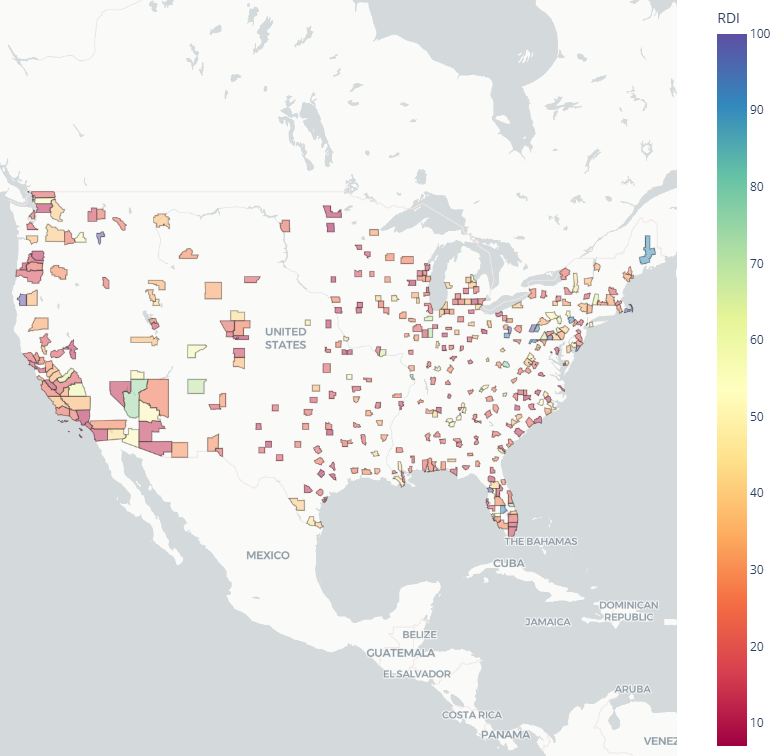
\includegraphics[width=\linewidth]{us.png}
		\caption{United States}\label{fig:us_choropleth}
	\end{subfigure}\hfill
	\begin{subfigure}[b]{0.32\textwidth}
		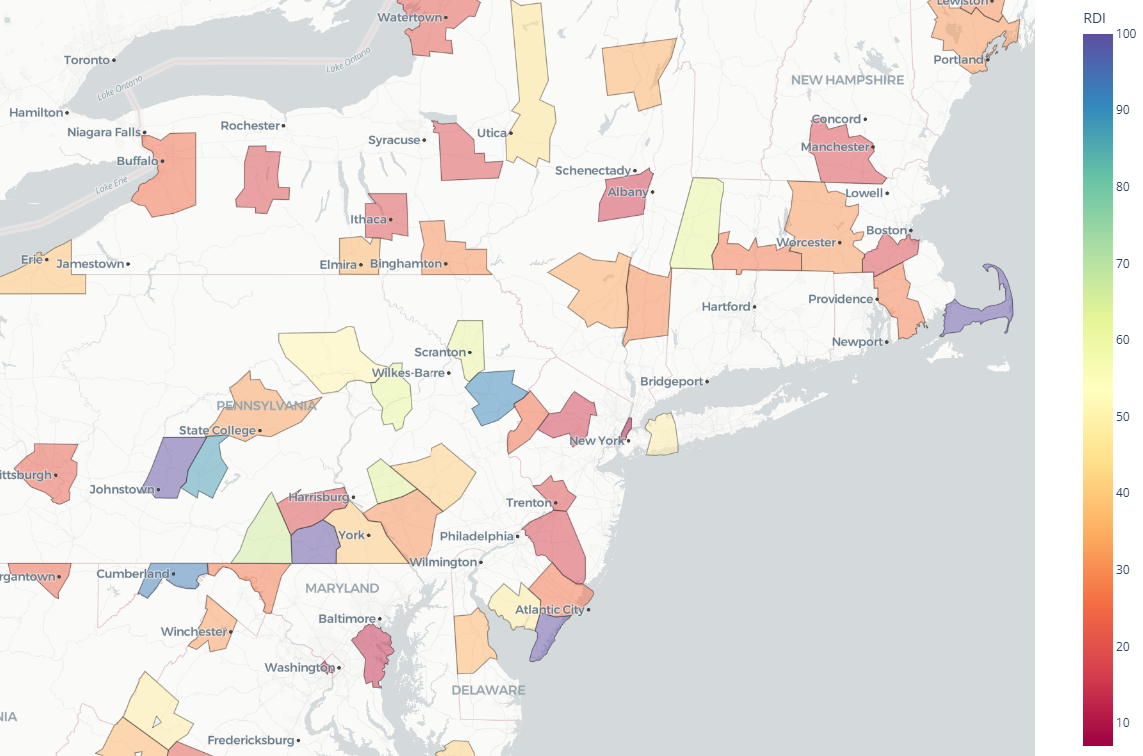
\includegraphics[width=\linewidth]{tristate.png}
		\caption{Tri-State area}\label{fig:tristate_choropleth}
	\end{subfigure}\hfill
	\begin{subfigure}[b]{0.32\textwidth}
		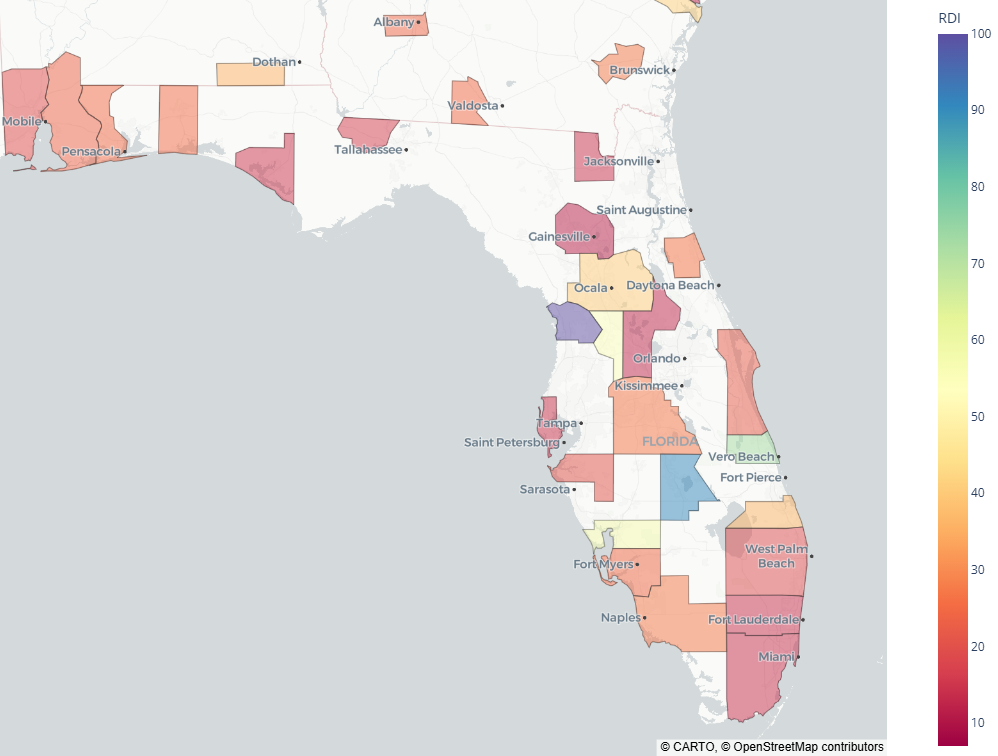
\includegraphics[width=\linewidth]{florida.png}
		\caption{Florida}\label{fig:florida_choropleth}
	\end{subfigure}
	
	\caption{Rental-Density-Index (RDI) choropleths at three spatial scales.}
	\label{fig:choropleth_panel}
\end{figure*}


While the RDI itself is useful for identifying how tight a market is at a given point in time, its absolute level is shaped by long-run demographic and structural trends such as rentership rates and changes in household formation. Accordingly, we focus on the \textit{year-over-year change in RDI}:

\begin{equation*}
	\Delta \text{RDI}_{it} = \text{RDI}_{it} - \text{RDI}_{it-1}.
\end{equation*}


The change in RDI (\( \Delta \text{RDI} \)) offers several advantages. First, it mitigates issues of nonstationarity in the level RDI, enabling cross-market comparison. Second, it reduces the impact of varying rentership percentages across cities. Most importantly, \( \Delta \text{RDI} \) captures demand pressure on housing stock: when it rises, it indicates more people are consolidating into fewer rental units, signaling tightening demand. When it falls, it implies renters are spreading out and absorbing more space, suggesting slack. It is useful to distinguish between two sources of crowding pressure captured by $\Delta \text{RDI}$: price-induced and supply-induced. Price-induced crowding occurs when rising rents outpace incomes, forcing renters to share space or delay household formation—behavioral responses that directly elevate RDI. Supply-induced crowding, by contrast, may arise even without rent escalation if housing stock fails to expand alongside population, resulting in more residents per unit out of sheer constraint. While these mechanisms are observationally similar, our framework implicitly captures both, interpreting $\Delta \text{RDI}$ as the revealed outcome of frictions between housing availability and household spatial preferences. In this way, RDI growth reflects excess demand pressures—regardless of whether they arise from affordability shocks or constrained supply.


Theoretically, under the assumption that renters prefer more space to less, the change in RDI reveals when prices are sufficiently high to induce cohabitation and when price relief allows individuals to live separately. Thus, \( \Delta \text{RDI} \), especially when combined with rent growth, helps identify periods of excess demand or slack and allows us to trace out implied demand curves. As we show later, this approach allows us to locate the intersection between demand and supply curves using observable outcomes.

It is important to note that \(\Delta \text{RDI}\) is conditioned on the rental population and does not explicitly capture shifts between renting and homeownership. In markets where tenure transitions are volatile—such as during periods of mortgage credit expansion or policy-driven ownership incentives—changes in RDI may partly reflect movement between tenures rather than intra-renter space consumption. For example, a declining RDI could reflect renters exiting into homeownership rather than an easing of rental crowding. While the vast majority of variation in \(\Delta \text{RDI}\) likely reflects household formation and consolidation behavior within the rental market, readers should interpret RDI-based signals with awareness of broader tenure context, especially in markets with known ownership volatility.

\subsection{Summary Statistics}
Table \ref{tab:summary_stats} provides descriptive statistics for the key variables across the full panel. On average, the RDI across all MSAs and years is approximately 2.31 persons per rental unit, with a standard deviation of 0.35. The average real rent per square foot is \$1.22, and the average annual growth in rental supply is 1.9\%. The missing records exist only in the beginning or ending years as the prior period and next-period values do not exist. 

\begin{table}[hbt!]
	\centering
	\caption{Summary Statistics (2000--2024)}\label{tab:summary_stats}
	\begin{tabular}{lrrrrrrrr}
	\toprule
	Variable & Mean       & Std.\ Dev.\   & Min       & 25th Pct.  & Median     & 75th Pct.  & Max        & Missing \\
	\midrule
	Population          & 2,012,976  & 2,169,231  &   175,653  &   758,060  & 1,224,731  & 2,422,333  & 14,849,020 &   0  \\
	Inventory           &   133,435  &   190,354  &    20,783  &    35,735  &    66,261  &   153,774  &  1,572,425 &   0  \\
	Supply growth       &      0.0169&      0.0152&     –0.0173&     0.0057 &    –0.0059 &     0.0239 &     0.1061 & 100  \\
	RDI                 &     18.259 &      6.852 &      6.841 &    13.737  &    17.067  &    20.967  &    64.795  &   0  \\
	RDI growth          &     –0.0078&      0.0151&     –0.1895&    –0.0163 &    –0.0059 &     0.0022 &     0.0512 & 100  \\
	Real rent (\$/sqft) &      0.9489&      0.3551 &      0.5584&     0.7164 &     0.8373 &     1.0436 &     2.9110 &   0  \\
	Real rent growth    &     –0.0035&      0.0300 &     –0.1915&    –0.0215 &    –0.0046 &     0.0114 &     0.2809 & 100  \\
	\bottomrule
\end{tabular}
\end{table}

\subsection{Coverage and Representativeness}
The sample includes approximately 1,300 MSA-year observations, covering a mix of large coastal cities, fast-growing Sun Belt metros, and slower-growing Midwestern regions. Together, these MSAs account for over 16 million of the 22 million U.S. apartment units, providing a representative snapshot of national rental dynamics. 

\subsection{Preliminary Observations}

Figure \ref{fig:sidebyside} traces the national Rental Density Index (RDI) from 2000 to 2024. Contrary to conventional wisdom about an acute housing shortage, we observe a steady decline in people per unit (from roughly 16 people-per-unit in 2000 to 13 people-per-unit in 2024). A companion histogram of ΔRDI is stationary but skewed slightly negative, confirming that most years see more units added per new person than vice versa.

\begin{figure}[!htb]
	\centering
	\begin{subfigure}[b]{0.48\textwidth}
		\centering
		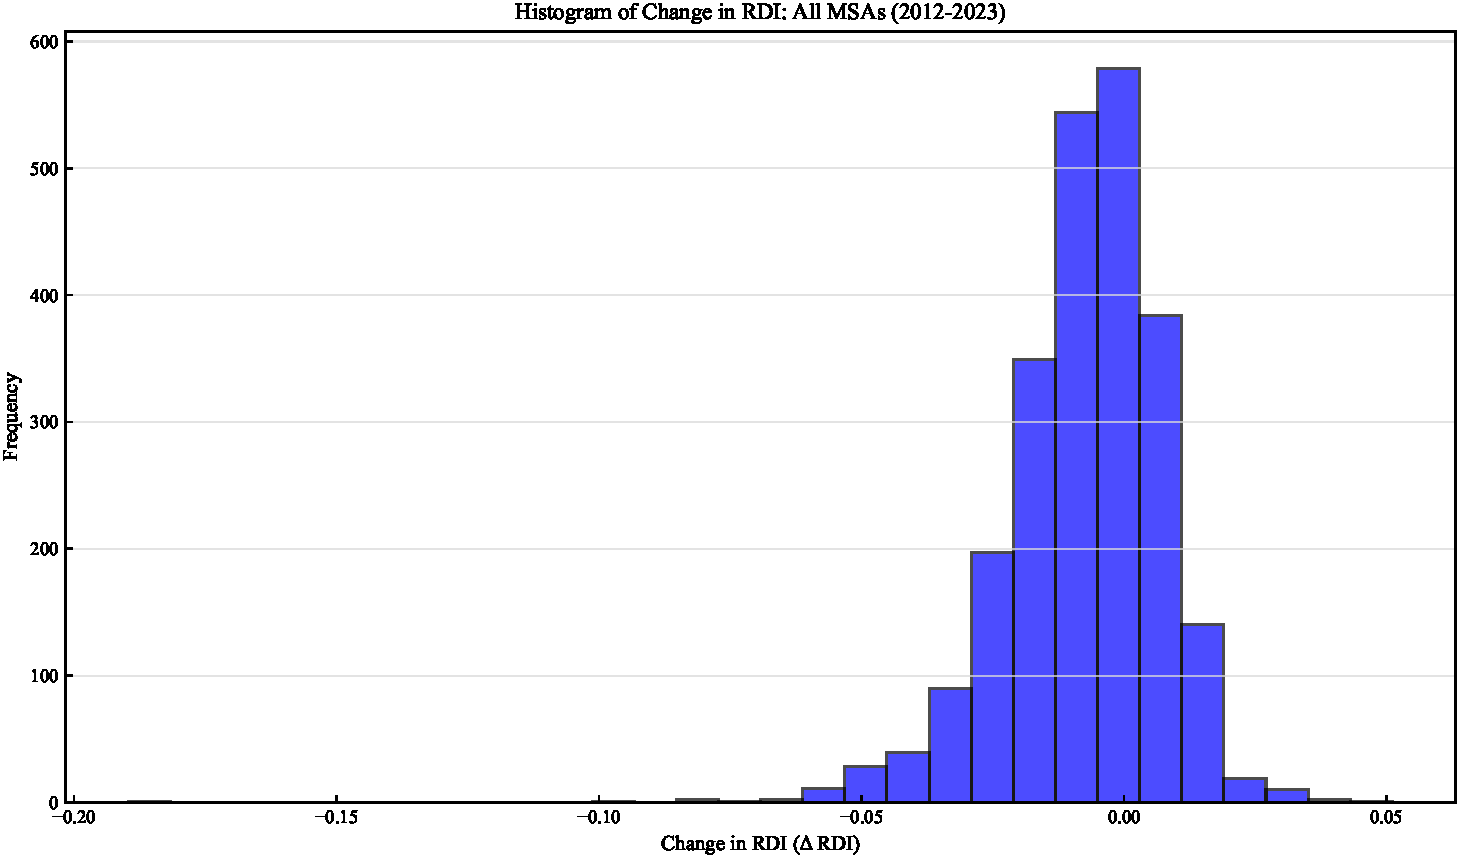
\includegraphics[width=\textwidth]{rdi_growth_histogram.pdf}
		\caption{A histogram of the annual change in RDI across 100 MSAs in the years 2001-2023. The outlier to the left is New  Orleans in 2004, due to Huricane Katrina.\label{fig:rdi_hist}}
	\end{subfigure}
	\hfill
	\begin{subfigure}[b]{0.48\textwidth}
		\centering
		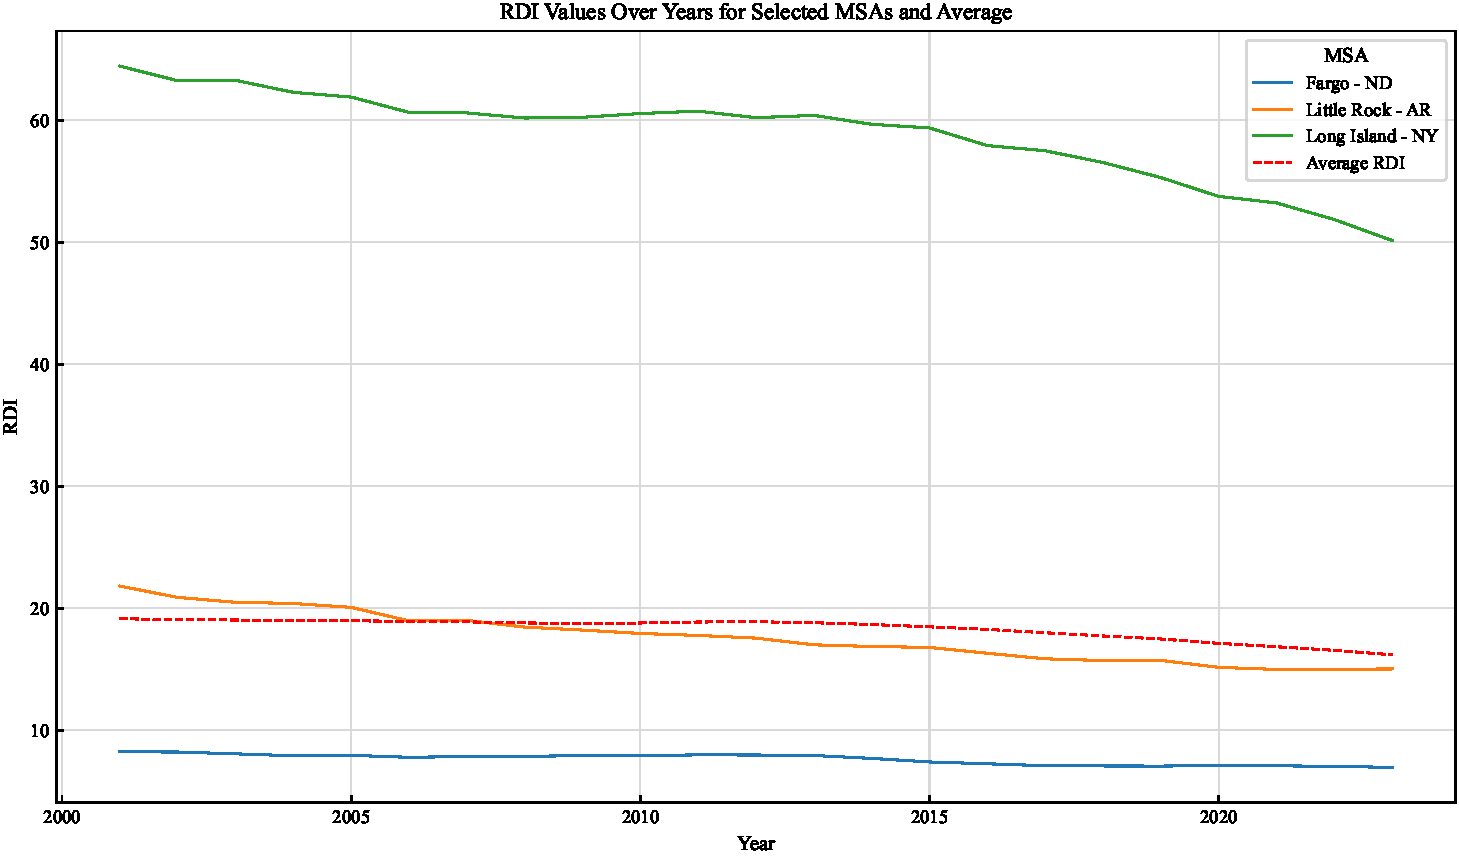
\includegraphics[width=\textwidth]{rdi_trends_selected_msas.pdf}
		\caption{A line graph showing the RDI values (population divided by apartment units) for the MSAs that were the min, max, and median in year 2001}
		\label{fig:rdi_lines}
	\end{subfigure}
	\caption{Histogram of Change in RDI, and Line Graph of RDI}
	\label{fig:sidebyside}
\end{figure}
This pattern poses a puzzle: if supply growth has outstripped population growth, why is everyone still worried about shortages? Occupancy simply tells you \textit{that} units are full--it cannot distinguish whether they are full by choice (everyone prefers roommates) or by necessity (everyone must share).

By contrast, year-over-year changes in RDI isolate the relative pace of new households versus new units. When rents rise faster than new construction can absorb, ΔRDI spikes, revealing latent demand pressure. When deliveries overwhelm demand, ΔRDI falls, signaling surplus. In the next section we exploit that property, regressing ΔRDI on rent and supply growth to recover the underlying demand curve.

\section{Empirical Strategy and Econometric Results}
\label{sec:instrumental-variable}

We estimate the causal effect of crowding—measured as the change in the Rental Density Index (\(\Delta \text{RDI}\))—on future rent growth using a two-stage least squares (2SLS) instrumental variables (IV) approach. This is necessary because \(\Delta \text{RDI}\) may be endogenous to unobserved demand shocks or simultaneous determination with rents. For example, rising rents may compress household formation (raising RDI), or latent shocks could affect both rents and occupancy intensity.

To isolate exogenous variation, we instrument \(\Delta \text{RDI}\) with foreign in-migration as a share of local population—capturing rare and plausibly unanticipated inflows. We implement two instrument definitions. In the continuous specification, \(\text{exog\_shock}_{it}\) is defined as the foreign in-migration share. In the binary specification, \(\text{exog\_shock}_{it} = 1\) when foreign in-migration exceeds 0.8\% of population—encompassing approximately 7.2\% of MSA-years—and 0 otherwise. To further support instrument validity, we test whether lagged rent growth predicts foreign in-migration share. We instrument $\Delta \text{RDI}_{it}$ using foreign in-migration as a share of the local population. We foundno significant relationship ($\beta = -0.415$, $p = 0.215$) in a fixed-effects panel regression. This supports the instrument’s exogeneity. This supports the assumption that foreign migration shocks are not driven by prior local rent trends and are plausibly exogenous to local rental market conditions. Details can be found in \ref{appendixa}

\begin{align*}
	\text{Stage 1:} \quad & \Delta \text{RDI}_{i,t} = \gamma_0 + \gamma_1 \cdot \text{Shock}_{i,t} + \gamma_2 \cdot \mathbf{X}_{i,t} + \mu_i + \delta_t + u_{i,t} \\\\
	\text{Stage 2:} \quad & \text{RentGrowth}_{i,t+1} = \alpha_0 + \beta \cdot \widehat{\Delta \text{RDI}}_{i,t} + \alpha_1 \cdot \mathbf{X}_{i,t} + \mu_i + \delta_t + \varepsilon_{i,t}
\end{align*}
Where:
\begin{itemize}
	\item $\text{RentGrowth}_{i,t+1}$ is next-year relative real rent growth in MSA $i$,
	\item $\Delta \text{RDI}_{i,t}$ is the change in Rental Density Index (crowding pressure),
	\item $\text{Shock}_{i,t}$ is the instrument—either foreign migration share (continuous) or high-migration indicator (binary),
	\item $\mathbf{X}_{i,t}$ includes controls: population growth and sales volume growth,
	\item $\mu_i$ and $\delta_t$ are MSA and year fixed effects.
\end{itemize}


Both specifications (continuous and binary) yield statistically significant and robust estimates. Using the continuous instrument, the estimated effect of \(\Delta \text{RDI}\) is 2.31 (\(p = 0.0010\)), with a strong first-stage F-statistic of 30.3. A placebo test, which replaces the outcome with contemporaneous rent growth, returns a smaller and weaker coefficient (1.66, \(p = 0.0019\)), consistent with a forward-looking interpretation.

Using the binary instrument, the estimated coefficient is 1.68 (\(p = 0.0173\)), with an F-statistic of 39.9. The placebo result remains significant but slightly attenuated (1.61, \(p = 0.0183\)). While the binary version benefits from a cleaner exclusion argument, the continuous specification provides stronger statistical power and supports robustness across specifications.

Results weaken when we use lagged instruments: neither the binary nor continuous lag yields statistically significant coefficients. This suggests that the migration–crowding relationship is contemporaneous, reflecting the immediacy of household absorption into rental stock.

\begin{table}[h]
	\centering
	\caption{Summary of 2SLS Estimates of $\Delta \text{RDI}$ on Next-Year Relative Rent Growth for both a Continuous and Binary Shock Variable}
	\label{tab:iv-summary}
	\begin{tabular}{lcccc}
		\toprule
		Instrument Type & Coef. on $\Delta$RDI & Std. Err. & $p$-value & F-stat (1st Stage) \\
		\midrule
		Continuous (contemp.) & 2.31 & 0.70 & 0.0010 & 30.3 \\
		Continuous (placebo)  & 1.66 & 0.53 & 0.0019 & 62.4 \\
		Binary (contemp.)     & 1.68 & 0.71 & 0.0173 & 39.9 \\
		Binary (placebo)      & 1.61 & 0.68 & 0.0183 & 62.9 \\
		Lagged (continuous)   & 1.54 & 0.86 & 0.0740 & 42.8 \\
		Lagged (binary)       & -0.35 & 1.02 & 0.7282 & 62.8 \\
		\bottomrule
	\end{tabular}
\end{table}

Together, these models confirm that exogenous migration shocks produce measurable increases in crowding pressure, and that these crowding effects reliably forecast future rent growth. All specifications include MSA and year fixed effects, ensuring that the estimated relationships are not confounded by time-invariant local characteristics or national-level shocks. The consistency of findings across instrument definitions and robustness checks strengthens confidence in \(\Delta \text{RDI}\) as a causal and timely proxy for rental housing demand.

While the IV model provides a causal estimate of the effect of crowding pressure on rent growth, the subsequent tests in Section~\ref{sec:forecasting-validation} evaluate whether \(\Delta \text{RDI}\) can serve as a useful predictive signal. These forecasting models do not claim to identify structural relationships, but rather assess the practical value of RDI for anticipating future market conditions.




\section{Forecasting Validation and Real-World Performance}
This section evaluates whether RDI functions as a useful predictive signal for rent growth, independent of causal identification. We organize the analysis into five complementary tests: (1) a simple group-wise ANOVA showing forward rent segmentation by RDI direction; (2) an event study evaluating rent dynamics before and after regime shifts in RDI; (3) a top-vs-bottom quintile spread comparison across forecasting models; (4) a long-horizon signal using count-based RDI persistence; and (5) a diagnostic of supply growth in context, showing how RDI mediates the impact of new supply. Together, these tests examine the predictive performance, durability, and explanatory clarity of RDI across diverse empirical contexts.

\subsection{Predictive Segment Testing: ANOVA on RDI Growth}
We test whether observed changes in RDI can segment markets into meaningful groups in terms of future rent performance. Specifically, we split the samples into two regimes: those with positive $\Delta$RDI and those negative $\Delta$RDI. We then examine whether average next-year relative real rent growth differs significantly across these groups.

Table~\ref{tab:anova-results} shows that markets with positive RDI growth experience average next-year rent growth of 41 basis points above the mean rent growth (significant at p$\leq 3.14^{-14}$), while markets with non-positive RDI growth exhibit an average decline of 15 basis points (significant at p$\leq$0.0026). The difference is statistically significant, as confirmed by both a one-way ANOVA and Tukey’s HSD post-hoc test.

\begin{table}[h]
	\centering
	\caption{ANOVA of Next Year's Relative Real Rent Growth Grouped by RDI}
	\label{tab:anova-results}
	\begin{tabular}{lcccccc} \toprule
		$\Delta$RDI Group & Mean (bps) & SE (bps) & 95\% CI Lower & 95\% CI Upper & $n$ & $p$-value \\ \midrule
		RDI Decline & -15 & 5 & -25 & -5 & 1538 & 0.0026 \\
		RDI Growth & 41 & 7 & 31 & 52 & 762 & $3.14^{-14}$ \\
		\bottomrule
	\end{tabular}
\end{table}

A two-way ANOVA confirms the significance of the group difference ($F = 49.2$, $p \leq 2.98 \times 10^{-12}$), and a Tukey HSD test further validates that the difference in means is statistically distinguishable.
\begin{table}[h]
	\centering
	\caption{Two-Way ANOVA Test Results}
	\label{tab:two-way-anova}
	\begin{tabular}{lcccc} \toprule
		Term & Sum Sq & DF & F & p-value \\ \midrule
		C(demand) & 0.0165 & 1.0 & 49.23 &  $2.98^{-12}$\\
		Residual & 0.7699 & 2298.0 & --- & --- \\
		\bottomrule
	\end{tabular}
\end{table}

\begin{table}[h]
	\centering
	\caption{Tukey HSD Test Results}
	\label{tab:tukey}
	
	\begin{tabular}{lcccccc} \toprule
		Group 1 & Group 2 & Mean Diff & p-adj & Lower & Upper & Reject \\ \midrule
		$\Delta$ RDI $\leq$0 & $\Delta$RDI>0 & 0.0057 & 0.0000 & 0.0041 & 0.0073 & True \\
		\bottomrule
	\end{tabular}
\end{table}

These results show that even without instrumentation, RDI growth serves as a powerful signal for forward rent performance. Practitioners can use RDI segmentation as a lightweight, interpretable classification rule for identifying tight rental markets.

\subsection{Event Study of RDI Regime Transitions}
We next evaluate how rent growth responds dynamically to transitions into and out of RDI-growth regimes. Specifically, we examine rent growth before and after a market switches into a state of positive  $\Delta$RDI (increasing crowding) or  negative  $\Delta$RDI (declining crowding). We continue to examine results in terms of real rent growth relative to the mean rent growth of that year, to avoid capturing rent changes due to macro conditions.

Figure~\ref{fig:event-study} illustrates rent growth over a five-year window centered on the regime switch. The blue line represents transitions into crowding markets, the red line transitions into de-densifying markets, and the gray line shows cases where RDI status does not change.

\begin{figure}[h]
	\centering
	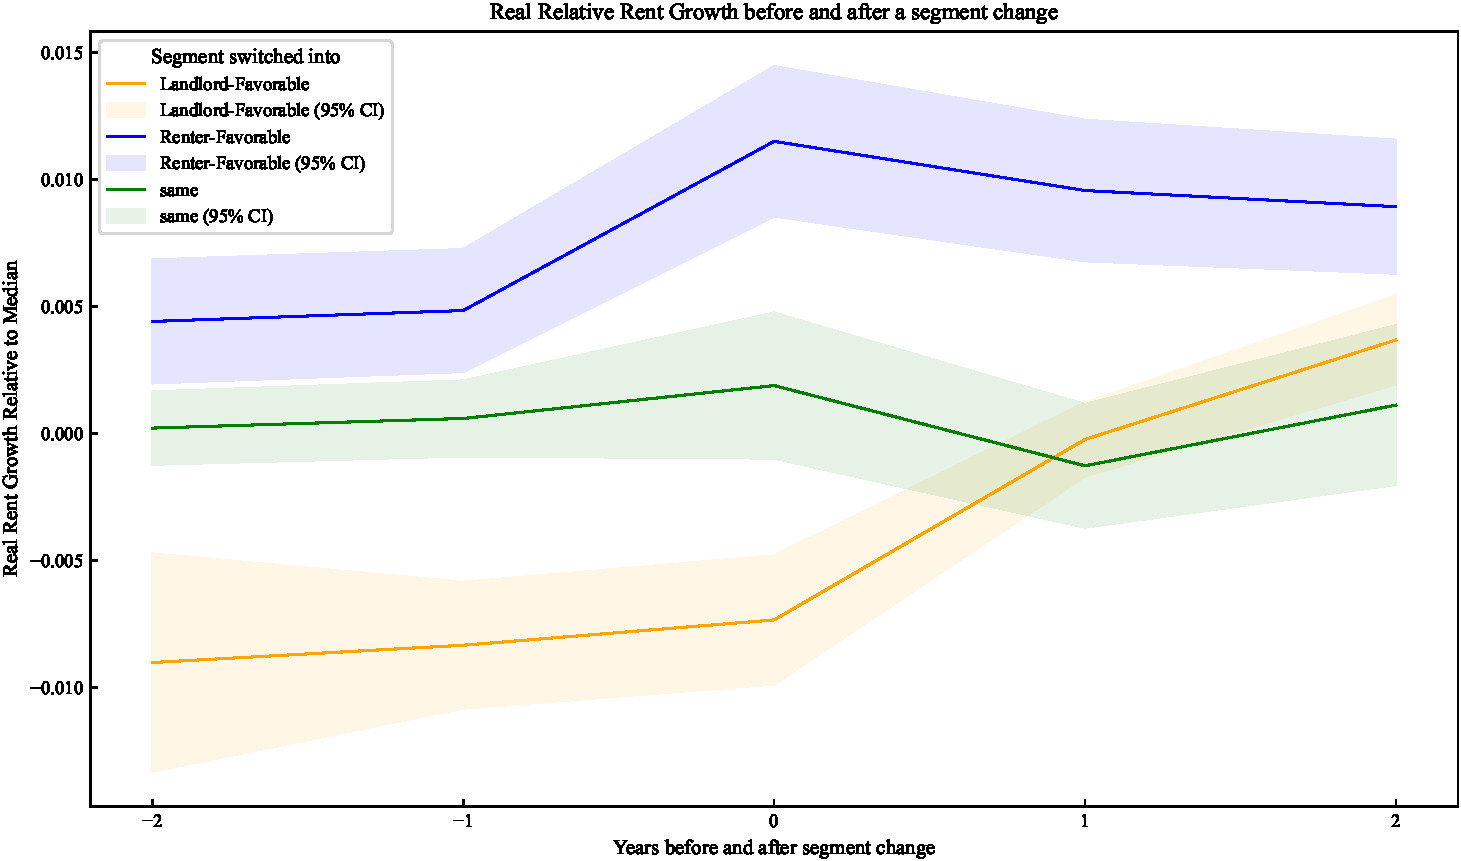
\includegraphics[width=0.8\textwidth]{event_study.pdf}
	\caption{Real Relative Rent Growth Before and After a Market Switches From/To Positive/Negative $\Delta$RDI}
	\label{fig:event-study}
\end{figure}

Table~\ref{tab:event-means} reports differences in average rent growth before and after the regime shift. Markets transitioning into crowded segments see a 48 basis point increase in rent growth, while those exiting see a 29 basis point decline. No significant change is observed when RDI status remains unchanged, as expected.

\begin{table}[h]
	\centering
	\caption{Mean Rent Growth Before and After RDI Regime Transition}
	\label{tab:event-means}
	\begin{tabular}{lcccc} \toprule
		Transition Type & Mean Before & Mean After & Difference & p-value\\ \midrule
		Switched to $\Delta \text{RDI}>0$ & -31 & 17 & 48 & 0.0027\\
		Switched to $\Delta \text{RDI}\leq0$ & 52 & 23 & -29 & 0.0089\\
		No change & -3 & -8 & -5 & 0.6336\\
		\bottomrule
	\end{tabular}
\end{table}

These dynamics confirm that the onset of crowding pressures, as measured by RDI, precedes statistically and economically meaningful changes in rent performance. RDI transitions can therefore serve as timely indicators of shifts in market pricing power.


\subsection{Forecast Spread Comparison: RDI vs ARIMA vs Naïve}
We compare the predictive strength of RDI growth against ARIMA-based and naive trailing average models in forecasting real rent growth across multiple time horizons. For each method, we rank MSAs into quintiles based on their predicted growth and compute the realized top-minus-bottom quintile spread.
Figure~\ref{fig:spread-comparison-quadrant} displays forecast accuracy over one-year, three-year, five-year, and ten-year windows. The RDI-based approach consistently delivers stronger spread segmentation, particularly at longer horizons where traditional time-series methods tend to degrade.

\begin{figure}[h!]
	\centering
	\begin{tabular}{cc}
		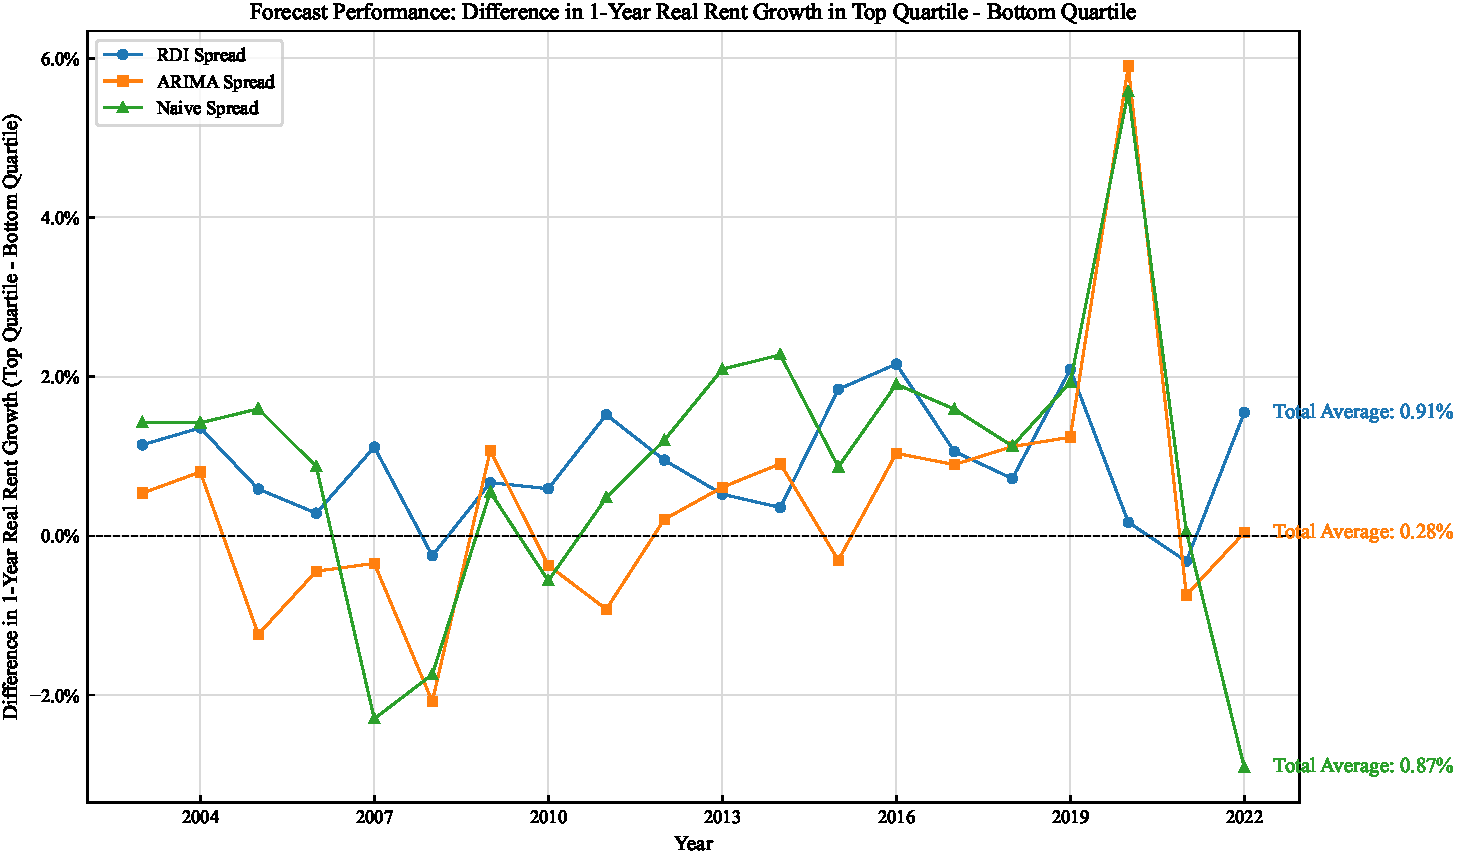
\includegraphics[width=0.45\textwidth]{spread_comparison_over_time_1yr.pdf} &
		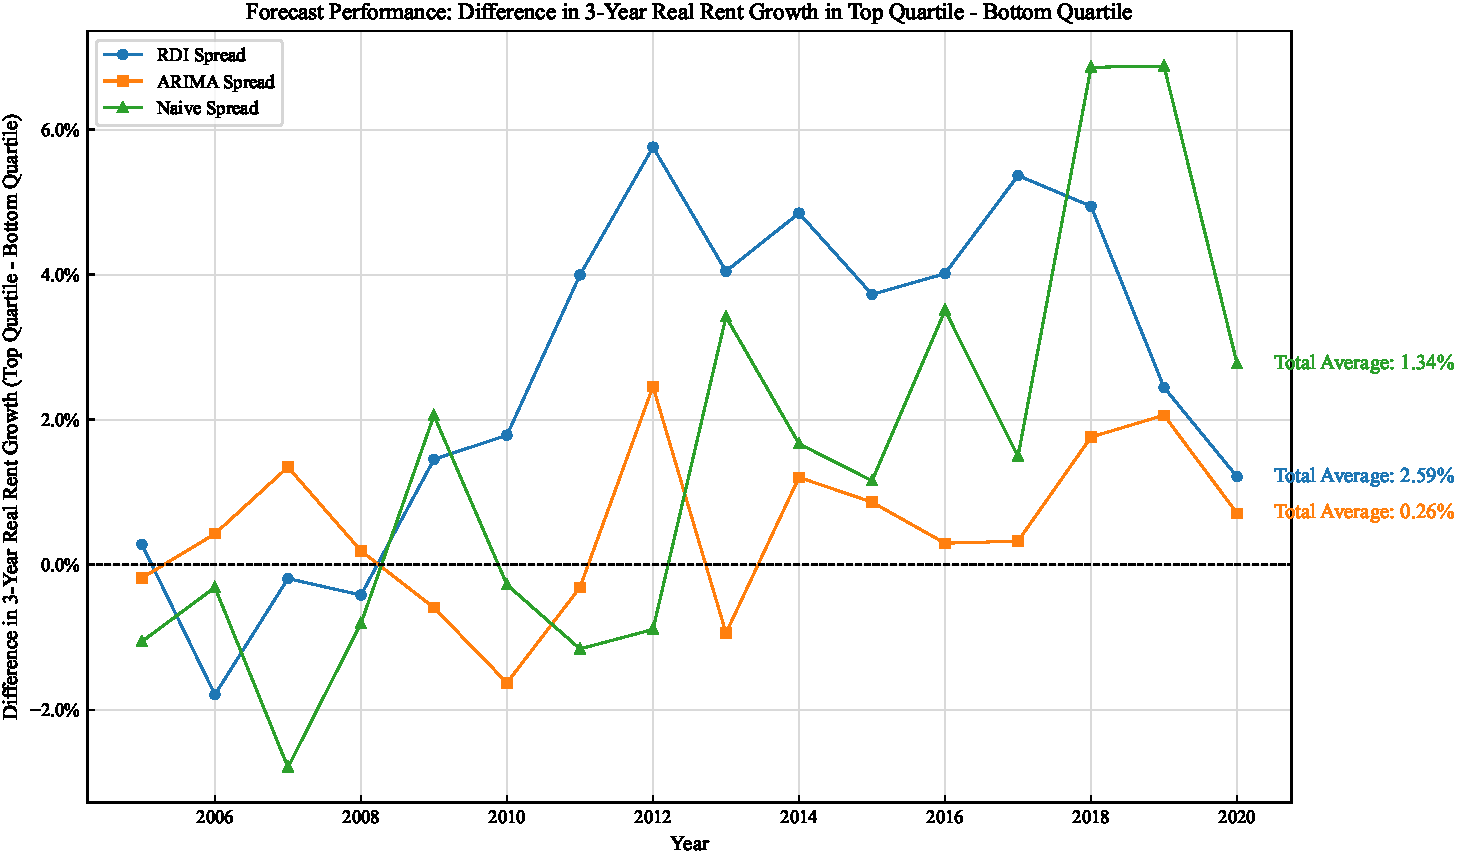
\includegraphics[width=0.45\textwidth]{spread_comparison_over_time_3yr.pdf} \\
		\textbf{(a)} 1-Year Forecast & \textbf{(b)} 3-Year Forecast \\
		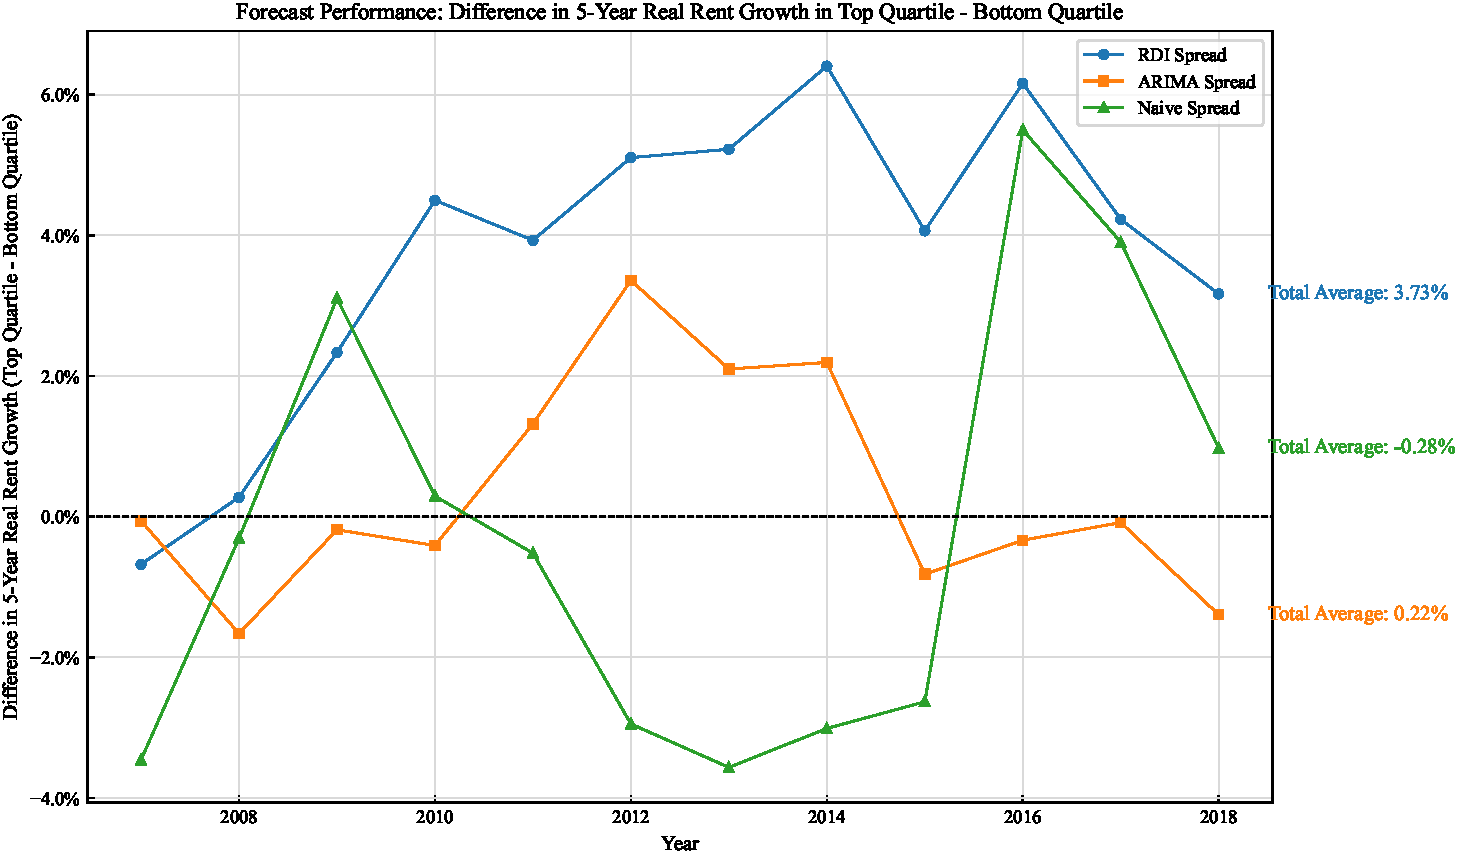
\includegraphics[width=0.45\textwidth]{spread_comparison_over_time_5yr.pdf} &
		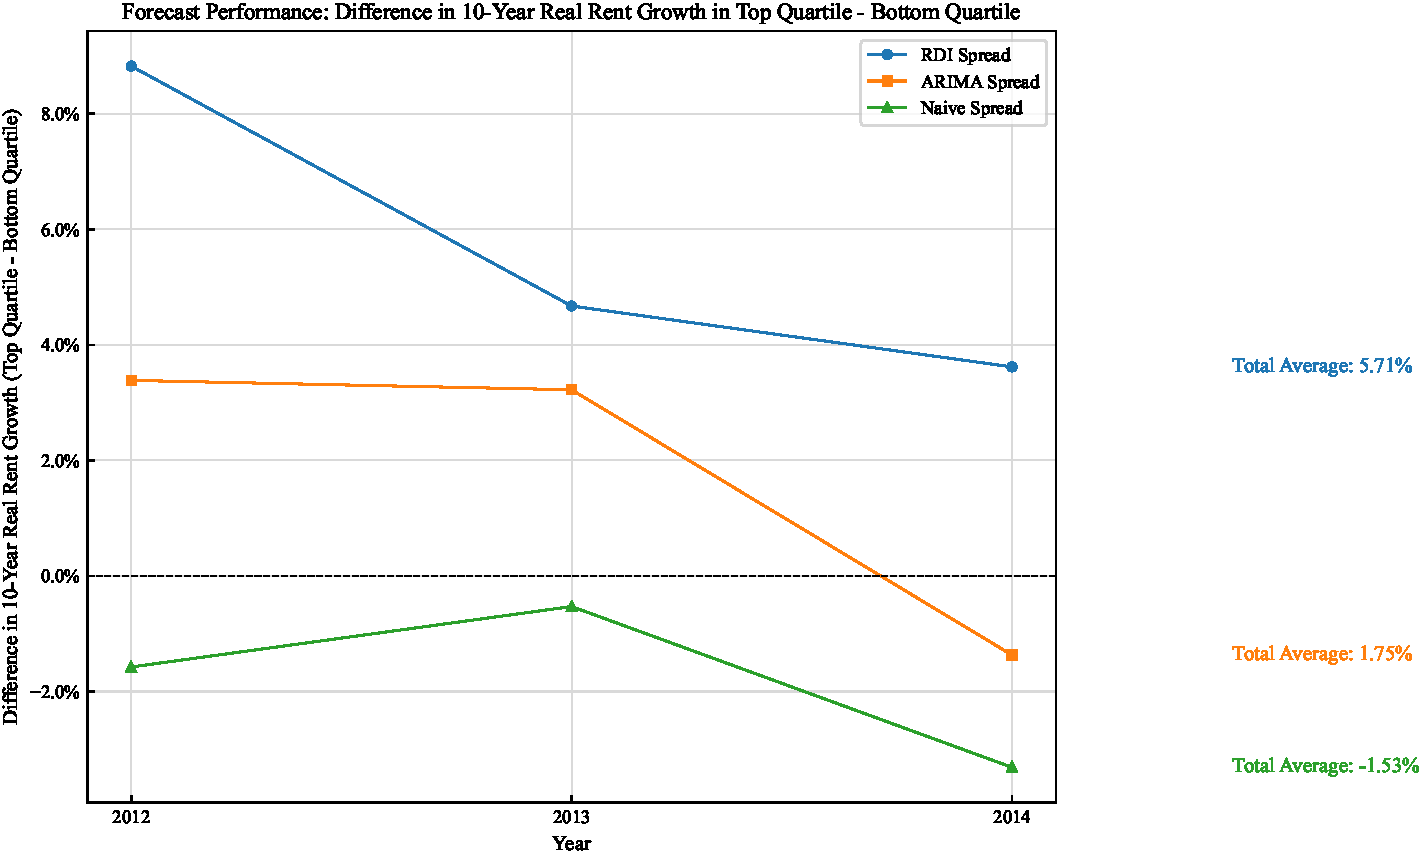
\includegraphics[width=0.45\textwidth]{spread_comparison_over_time_10yr.pdf} \\
		\textbf{(c)} 5-Year Forecast & \textbf{(d)} 10-Year Forecast \\
	\end{tabular}
	\caption{Top-minus-Bottom Quintile Rent Growth Spread by Forecast Method and Horizon}
	\label{fig:spread-comparison-quadrant}
\end{figure}

These results reinforce the value of RDI as not only a causal explanatory variable but also a forward-looking predictive signal. Forecasting long-term rent growth is notoriously difficult; most models lose power beyond a few years. The fact that the RDI-based approach maintains signal strength across one-, three-, five-, and ten-year periods underscores its robustness. While time series models rely on trailing trends, RDI captures forward-looking, structural occupancy pressure—making it an effective long-horizon indicator of underlying demand.

\subsection{RDI Positivity Persistence and Long-Term Rent Growth}
We test whether a simple count of trailing years with positive RDI growth serves as a meaningful predictor of future rent appreciation. Specifically, we examine the relationship between the number of years in which  over trailing five- and ten-year windows, and cumulative real rent growth over the subsequent five and ten years, respectively.

Figure~\ref{fig:rdi-counts} shows a clear, monotonic relationship: markets with more consistent positive RDI observations tend to experience stronger future rent growth. This pattern holds across both time horizons and supports the argument that RDI functions as a persistent, structural signal of housing demand.

\begin{figure}[h]
	\centering
	\begin{tabular}{cc}
		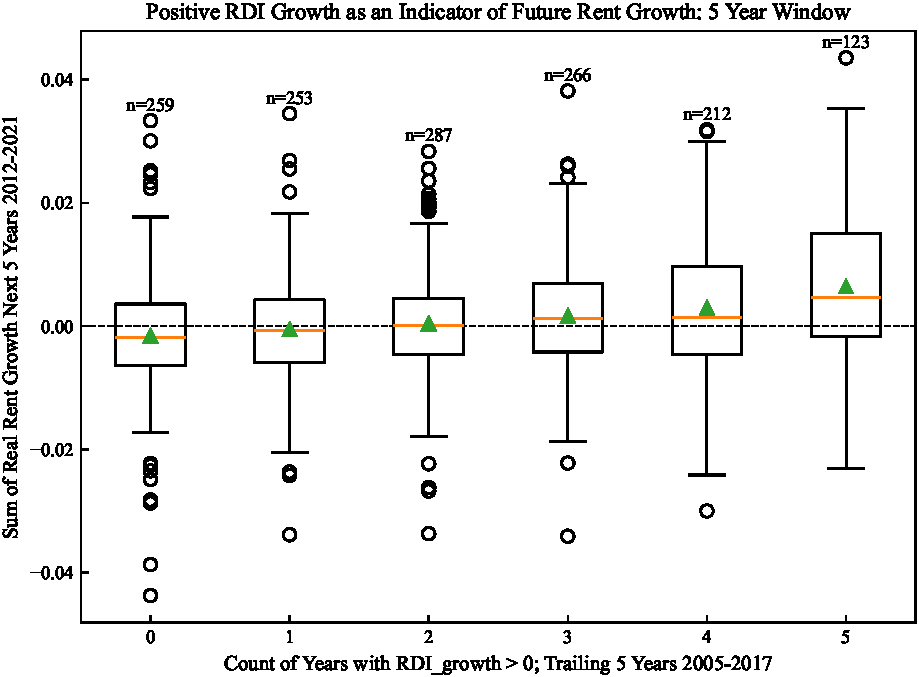
\includegraphics[width=0.45\textwidth]{rdi_positive_counts_vs_rent_growth_5yr.pdf} &
		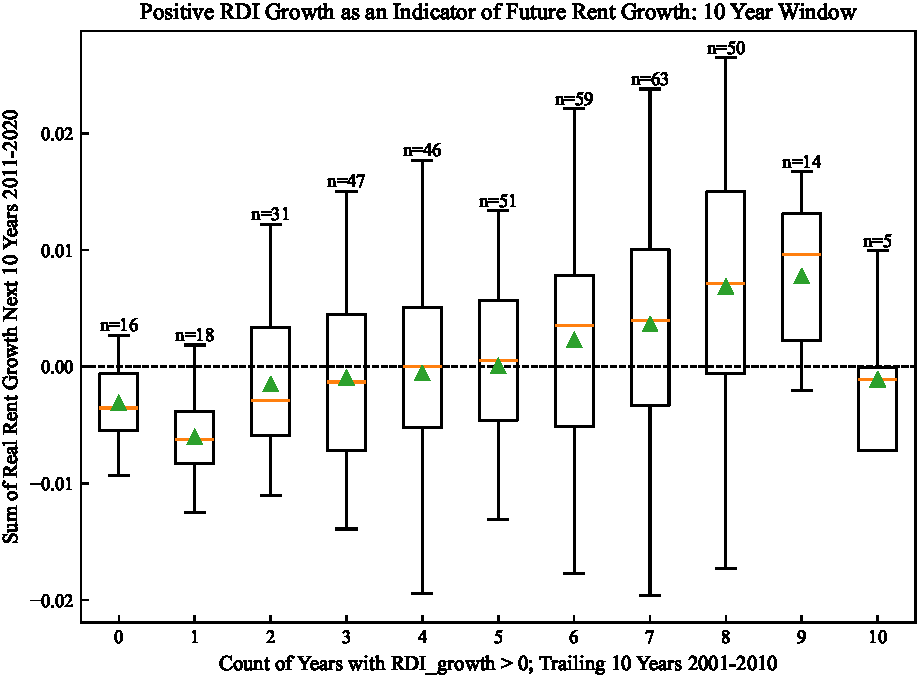
\includegraphics[width=0.45\textwidth]{rdi_positive_counts_vs_rent_growth_10yr.pdf} \\
		\textbf{(a)} 5-Year Horizon & \textbf{(b)} 10-Year Horizon \
	\end{tabular}
	\caption{Cumulative Rent Growth by Number of Positive RDI Years in Prior Window}
	\label{fig:rdi-counts}
\end{figure}

These results reinforce the practical utility of RDI: even without complex forecasting models, the persistence of positive RDI signals—interpreted as consistent crowding pressure—can help classify markets by likely long-term pricing strength.

\subsection{Supply Growth in Context: RDI as a Mediating Lens}
It is often assumed that elevated supply growth should depress rents in subsequent years. To test this assumption, we identify each MSA's year of maximum supply growth and examine the subsequent year’s real relative rent growth. Figure~\ref{fig:supply-rent} shows that the relationship is weak: nearly 45% of markets still experienced positive rent growth even after their peak supply year, and the overall correlation is low ().

In contrast, when we examine how RDI responds in those same years (Figure~\ref{fig:supply-rent}b), the relationship between supply growth and RDI growth is clearer. This suggests that crowding pressures, not raw supply levels, better mediate subsequent rent performance. Even in high-supply environments, strong demand absorption (captured by RDI) can offset what might otherwise appear to be oversupply conditions.

\begin{figure}[h]
	\centering
	\begin{tabular}{cc}
		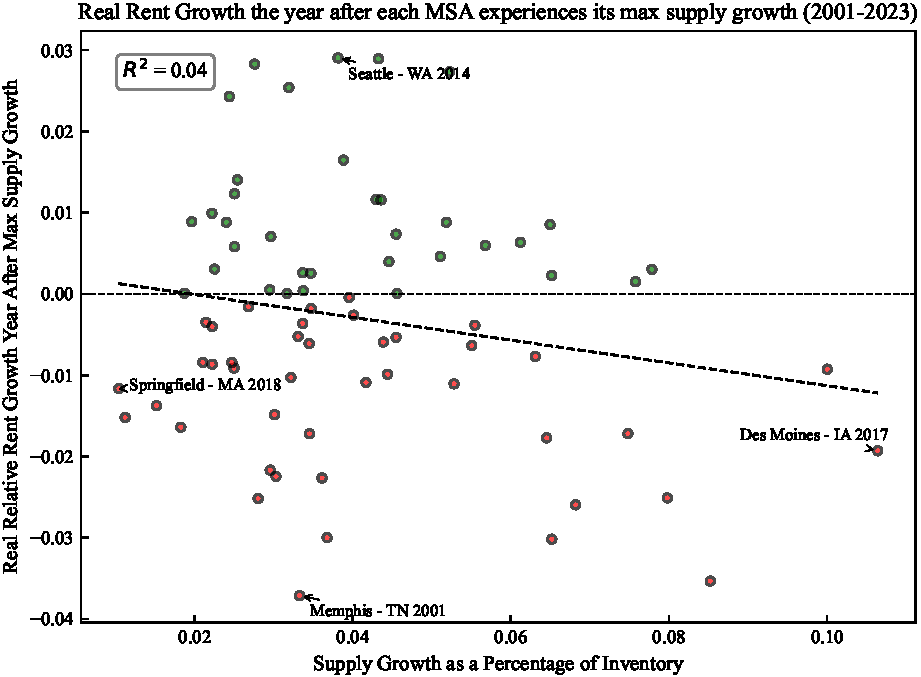
\includegraphics[width=0.45\textwidth]{max_supply_growth_vs_rent_growth.pdf} &
		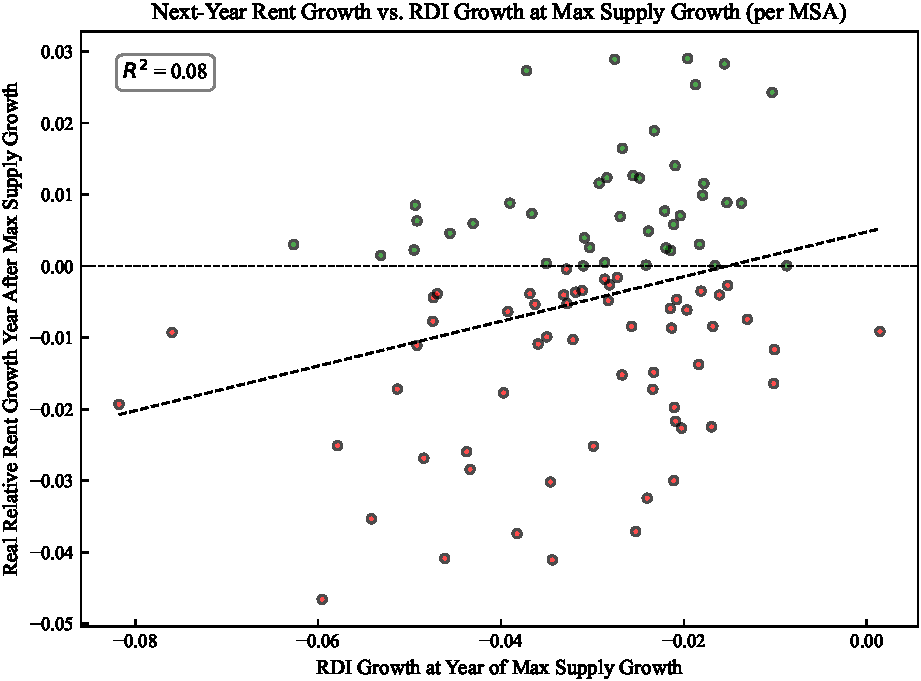
\includegraphics[width=0.45\textwidth]{max_supply_vs_RDI_growth.pdf} \\
		\textbf{(a)} Supply Growth vs. Subsequent Rent Growth & \textbf{(b)} Supply Growth vs. RDI Growth \
	\end{tabular}
	\caption{Crowding Absorption During Maximum Supply Years}
	\label{fig:supply-rent}
\end{figure}

These results challenge the assumption that supply growth alone determines rent dynamics. Without considering how supply is absorbed relative to household formation, analysts risk misclassifying healthy markets as oversupplied. RDI offers a more reliable, demand-sensitive lens.

\subsection{Conclusion: RDI as a Practically Useful, Predictively Durable Demand Metric}
The empirical tests in this section demonstrate that RDI---a simple, observable measure of household crowding---delivers meaningful insight into rental market behavior. Across multiple frameworks, RDI consistently outperforms: it segments markets with forward---looking rent divergence, anticipates regime transitions, and reveals demand absorption dynamics even during peak supply years.

These results complement the causal identification strategy in Section~\ref{sec:instrumental-variable}, where instrumented RDI growth was shown to drive future rent increases. Here, we show that RDI also performs well in practice without instrumentation, making it suitable for real-time forecasting, benchmarking, and investment decisions.

While RDI is not without limits—its precision may weaken in data-sparse MSAs or highly regulated rent environments—it stands out as a behaviorally grounded, interpretable, and statistically durable signal of latent housing demand.


\section{Discussion}

This paper demonstrates that crowding pressure—captured by changes in the Rental Density Index ((\(\Delta\text{RDI}\)))—is a consistent and forward-looking indicator of rental market tightness. Across a range of empirical tests, we show that (\(\Delta\text{RDI}\)) segments markets into meaningfully different regimes, predicts future rent growth, and reveals the hidden intensity of demand even when traditional metrics appear stable. This paper distinguishes between two uses of RDI: as a causal driver of future rent growth, and as a predictive signal for practical forecasting. While our IV models establish the former, the forecasting results show that \(\Delta \text{RDI}\) retains value even outside a fully identified structural framework. That robustness—across both causal and predictive contexts—is a key strength of the RDI approach.

\subsection{Advantages}
Unlike static indicators such as occupancy or absorption, (\(\Delta\text{RDI}\)) reflects household behavioral responses to constrained housing supply, such as roommate formation, deferred household creation, or increased unit turnover. These signals often manifest before rents begin rising, making (\(\Delta\text{RDI}\)) particularly valuable as a leading indicator.

We find that (\(\Delta\text{RDI}\)) alone—and especially when evaluated alongside contemporaneous supply growth—can classify markets into distinct quadrants of demand-supply imbalance, with predictive implications for future rent performance. This classification aligns with fundamental housing economics: markets that are simultaneously undersupplied and overpriced show the strongest subsequent rent growth, while oversupplied and underpriced markets underperform.

Perhaps most notably, (\(\Delta\text{RDI}\)) retains its predictive power even in simple, out-of-sample frameworks. It outperforms both ARIMA and naive trailing average models across multiple forecasting horizons, including ten-year forward rent growth—an especially demanding test. Persistence of positive (\(\Delta\text{RDI}\)) also serves as a robust long-horizon signal, and we show that (\(\Delta\text{RDI}\)) better explains rent outcomes during peak-supply years than supply growth alone.

These results suggest that (\(\Delta\text{RDI}\)) is not only a descriptive measure of market pressure, but also a structurally grounded and practically useful forecasting tool. Its simplicity and scalability make it suitable for repeated, cross-market applications, especially where data or resources for full structural modeling are limited.

\subsection{Limitations: Tenure Shifts and Spatial Spillovers}

While RDI offers a parsimonious and scalable indicator of rental demand pressure, it is important to acknowledge two interpretive limitations. First, the framework assumes a stable tenure composition—i.e., that observed changes in population per occupied rental unit reflect shifts within the renter segment. However, in some markets, changes in RDI may be partially driven by tenure transitions, such as households moving into homeownership or into rental units from ownership due to credit constraints or housing cost burdens. For example, a declining RDI might suggest easing crowding pressure, but could also reflect renter outmigration into the owner-occupied segment. Conversely, increasing RDI may reflect ownership lock-in effects or affordability barriers that delay household formation. While these effects likely operate at the margin in most MSAs, acknowledging tenure fluidity is important for fully interpreting RDI-based signals. Future work could extend the RDI framework by incorporating tenure transition data or endogenizing homeownership trends.

Second, the current analysis treats each metropolitan statistical area (MSA) as an independent unit. In practice, however, housing market conditions are rarely contained by administrative boundaries. Migration, affordability spillovers, and commuting patterns often link neighboring MSAs, meaning that crowding pressures in one region may affect rental markets in adjacent areas. Ignoring these spillover dynamics may understate the correlated nature of demand shifts, especially in highly integrated urban corridors. Incorporating spatial dependence structures or spatially lagged RDI variables in future work may enhance model precision and improve detection of regional displacement or diffusion effects.

While we do not formally estimate a spatial lag model, we assess geographic clustering by examining pairwise correlations in $\Delta \text{RDI}$ across neighboring MSAs. We find strong co-movement among regionally linked markets—e.g., New York and Northern New Jersey ($r = 0.70$), San Francisco and San Jose ($r = 0.69$), and Dallas–Fort Worth and Austin ($r = 0.77$). These results suggest that crowding pressures often evolve in tandem across proximate metros, reflecting regional migration flows, shared housing constraints, or price spillovers. Future work could formalize these relationships using spatial dependence structures or migration-network adjacency matrices.




\section{Conclusion}

We propose the Rental Density Index (RDI) as a demand-centric metric for measuring latent pressure in multifamily rental markets. By tracking changes in population per occupied unit, RDI captures household-level crowding dynamics that precede and predict future rent movement. Our empirical results, validated across causal models, forecasting tests, and event studies, establish (\(\Delta\text{RDI}\)) as both a leading indicator and a practical classification tool.

The simplicity of RDI is a strength. While traditional demand estimation often requires detailed demographic or income data, RDI can be computed with widely available population and housing stock data. Yet it performs comparably—if not better—than more complex models, especially over long forecast horizons. It is also behaviorally grounded: renters adjust space usage when pricing becomes constrained, and this adjustment leaves measurable traces in the data.

Future research may extend this work in several directions. RDI could be evaluated alongside migration flows, income segmentation, or micro-level leasing data to refine its predictive specificity. It may also prove useful in pricing models, rent control policy evaluation, or early-warning systems for affordability crises.

In sum, this paper offers both a new way to quantify housing demand and a practical framework for translating that signal into market insight. (\(\Delta\text{RDI}\)) helps bridge the gap between structural economics and applied decision-making—and in doing so, offers analysts, policymakers, and investors a grounded, interpretable, and scalable tool for anticipating market behavior.

\section*{Appendix A: Instrument Validity}
\label{sec:appendixa}

To assess the exogeneity of our instrument, we test whether lagged relative rent growth predicts the share of foreign in-migration. We estimate:

\[
\text{foreign\_migration\_share}_{i,t} = \alpha + \beta \cdot \text{RentGrowth}_{i,t-1} + \gamma \cdot \textbf{X}_{i,t} + \mu_i + \delta_t + \varepsilon_{i,t}
\]

where $\textbf{X}_{i,t}$ includes population growth and sales volume growth, and $\mu_i$ and $\delta_t$ represent MSA and year fixed effects. The coefficient on lagged rent growth is statistically insignificant ($\beta = -0.415$, $p = 0.215$), providing support for the orthogonality of foreign migration shocks to prior local rent conditions.
\section*{Appendix B: Spillover Effect Correlation Matrix}
\begin{table}[h]
	\centering
	\caption{Cross-MSA Correlation in $\Delta \text{RDI}$ Among Regional Pairs}
	\label{tab:regional_corr}
	\begin{tabular}{lcc}
		\toprule
		MSA 1 & MSA 2 & Correlation ($r$) \\
		\midrule
		New York, NY & Northern New Jersey, NJ & 0.70 \\
		San Francisco, CA & San Jose, CA & 0.69 \\
		Dallas–Fort Worth, TX & Austin, TX & 0.77 \\
		Los Angeles, CA & Inland Empire, CA & 0.52 \\
		Miami, FL & Palm Beach, FL & 0.54 \\
		\bottomrule
	\end{tabular}
\end{table}


%\backmatter
\bmsection*{Author contributions}

All authors contributed equally

\bmsection*{Acknowledgments}


\bmsection*{Financial disclosure}

\bmsection*{Conflict of interest}


\bmsection*{Data Disclosure}


\bibliography{wileyNJD-APA}
\bmsection*{Supporting information}

Additional supporting information may be found in the
online version of the article at the publisher’s website.










\nocite{*}% Show all bib entries - both cited and uncited; comment this line to view only cited bib entries;


\end{document}
